\section{Durchführung}
\label{sec:Durchführung}

\subsection{Magnetfeld einer langen und kurzen Spule}
Zur Bestimmung des Magnetfeldes einer langen und kurzen Spule, werden jene an ein Netzgerät angeschlossen, wie in Abbildung (3) dargestellt ist.
Der maximal zulässige Strom für die Spulen beträgt $I_\text{max} = 1,4 \si{\ampere}$. 
Eine longitudinale Hall-Sonde wird zum Messen verwendet, und es werden innerhalb und außerhalb der Spulen Messwerte genommen. 
Die Windungszahl der Spulen beträgt $n = 300$.
\begin{figure}[H]
  \centering
  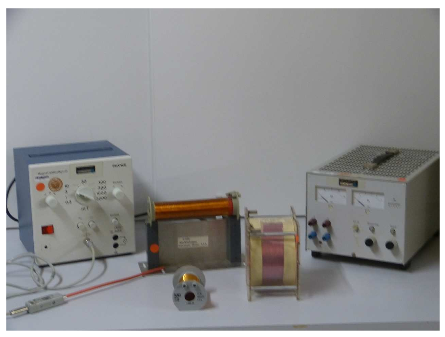
\includegraphics[height=5cm]{eins.png}
  \caption{Versuchsaufbau zur Messung des Magnetfelds einer Spule. \cite[S. 4]{sample}}
\end{figure}
\subsection{Magnetfeld eines Helmholtzspulenpaares}
Das Netzgerät wird an das Spulenpaar in Reihe angechlossen und der Strom wird so eingestellt, dass er $5 \si{\ampere} $ nicht überschreitet.
Es werden für 2 verschiedene Spulenabstände innerhalb und außerhalb Messwerte genommen. Für einen Abstand wird die Stromstärke einmal verändert und die gleiche Messreihe wiederholt.
Ein Aufbau ist in Abbildung (4) dargestellt. Beide Spulen haben eine Windungszahl von $n=100$, einen Durchmesser von $d=125 \si{\milli\meter}$ und eine Breite von $b=33 \si{\milli\meter}$.
\begin{figure}[H]
  \centering
  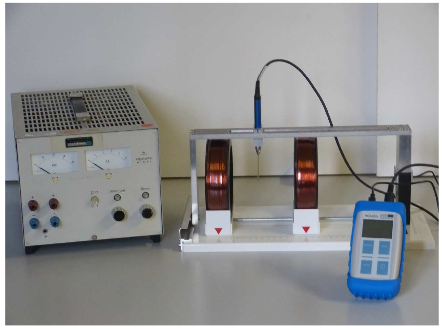
\includegraphics[height=5cm]{zwei.png}
  \caption{Versuchsaufbau zur Messung des Magnetfelds eines Helmholtzspulenpaares. \cite[S. 5]{sample}}
\end{figure}
\subsection{Bestimmung einer Hysteresekurve}
Das Netzgerät wird an die Ringspule angeschlossen und es werden mit einer transversalen Hall-Sonde Werte für das Magnetfeld bestimmt.
Dabei wird der Strom von $0$ auf $10$ Ampere hochgeregelt, dann runter auf $-10$ Ampere und wieder hoch auf $10$ Ampere gestellt. Es wird in Ein-Ampere-Schritten gemessen, also insgesamt $51$ Messwerte fürs Magnetfeld aufgenommen.
Abbildung (5) zeigt den Aufbau dieses Versuchsteils. Die Windungszahl der Ringspule ist $n = 595$.
\begin{figure}[H]
  \centering
  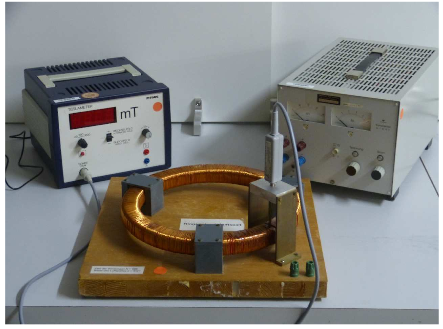
\includegraphics[height=5cm]{drei.png}
  \caption{Versuchsaufbau zur Messung des Magnetfelds einer Toroidspule. \cite[S. 5]{sample}}
\end{figure}